%%%%%%%%%%%%%%%%%%%%%%%%%%%%%%%%%%%%%%%%%%%%%%%%%%%%%%%%%%%%%%%%%%%%%%
% How to use writeLaTeX: 
%
% You edit the source code here on the left, and the preview on the
% right shows you the result within a few seconds.
%
% Bookmark this page and share the URL with your co-authors. They can
% edit at the same time!
%
% You can upload figures, bibliographies, custom classes and
% styles using the files menu.
%
%%%%%%%%%%%%%%%%%%%%%%%%%%%%%%%%%%%%%%%%%%%%%%%%%%%%%%%%%%%%%%%%%%%%%%

\documentclass[12pt]{article}

\usepackage{sbc-template}

\usepackage{graphicx,url}

%\usepackage[brazil]{babel}   
\usepackage[utf8]{inputenc} 

\usepackage{float}
\usepackage{hyperref}

\usepackage{listings}
\usepackage{color}

\definecolor{dkgreen}{rgb}{0,0.6,0}
\definecolor{gray}{rgb}{0.5,0.5,0.5}
\definecolor{mauve}{rgb}{0.58,0,0.82}

\lstset{frame=none,
  language=C++,
  aboveskip=3mm,
  belowskip=3mm,
  showstringspaces=false,
  columns=flexible,
  basicstyle={\small\ttfamily},
  numbers=none,
  numberstyle=\tiny\color{gray},
  keywordstyle=\color{blue},
  commentstyle=\color{dkgreen},
  stringstyle=\color{mauve},
  breaklines=true,
  breakatwhitespace=true,
  tabsize=3
}

     
\sloppy

\title{Deep Sleep}

\author{Fabricio Araújo Dias}

\address{Instituto Federal de Educação, Ciência e Tecnologia do Ceará
  (IFCE)\\
  Avenida Vice-Presidente José Alencar, S/N -- 61.939-140 -- Maracanaú -- CE -- Brasil
  \email{fabricio.araujo61@aluno.ifce.edu.br}
}

\begin{document} 

\maketitle

\begin{abstract}
  This report explains the steps taken to demonstrate the use of Deep Sleep on the ESP32. To test it, we made it so that when you touch one of the microcontroller's touch pins, it wakes up and lights a simple LED.
\end{abstract}
     
\begin{resumo} 
  Esse relatório explica os passos dados para exemplicar o uso do \textit{Deep Sleep} no ESP32. Para testá-lo, fizemos com que ao tocar em um dos pinos de \textit{touch} do microcontrolador, ele desperte e acenda um LED simples.
\end{resumo}


\section{Introdução}\label{sec:introdução}
A quinta atividade prática consiste primariamente em explorar o modo \textit{deep sleep} do ESP32. Esse modo consiste em deixar o ESP32 funcionando, mas com um consumo muito baixo, visando economizar energia e outros recursos. Quando for necessário, o ESP32 irá "acordar" e executar alguma instrução antes de "dormir" novamente.

Para demonstrar, iremos programar o ESP32 para que fique no modo \textit{deep sleep} e, por meio de um touch, acorde e acenda um LED simples, e logo depois, volte a dormir.

\section{Configuração no ESP32}

Começamos preparando os componentes. Vamos utilizar um ESP32 de 30 pinos, uma protoboard de 400 pontos, três cabos macho-fêmea, um resistor e um LED simples.

Primeiro, colocamos o LED num ponto qualquer da protoboard. Deixamos o seu terminal positivo em um ponto que fica próximo das linhas da protoboard, onde iremos ligar o seu terminal negativo. Na mesma coluna onde ligamos o terminal positivo do LED, instalamos um resistor de 390 ohms. Ele poderia dispor numa mesma coluna, mas resolvemos deixar um terminal na coluna do LED e o outro terminal numa outra coluna.

Iremos, então, ligar o ESP32 à protoboard. Escolhemos arbitrariamente o pino 25 para que seja conectado ao LED. Isto é, nós os conectamos através do resistor por meio de um cabo macho-fêmea. Utilizando outro cabo desse tipo, conectamos a linha negativa da protoboard, onde está o terminal negativo do LED, para o GND do ESP32.

Sobrou apenas utilizar um cabo macho-fêmea para conectar a algum pino de \textit{touch} do ESP32 e utilizar o lado macho do cabo para que sirva como touch. Conferindo o \textit{pinout} do ESP32 para descobrir quais são os seus pinos de \textit{touch}, escolhemos o pino 15.

\begin{figure}[H]
    \centering
    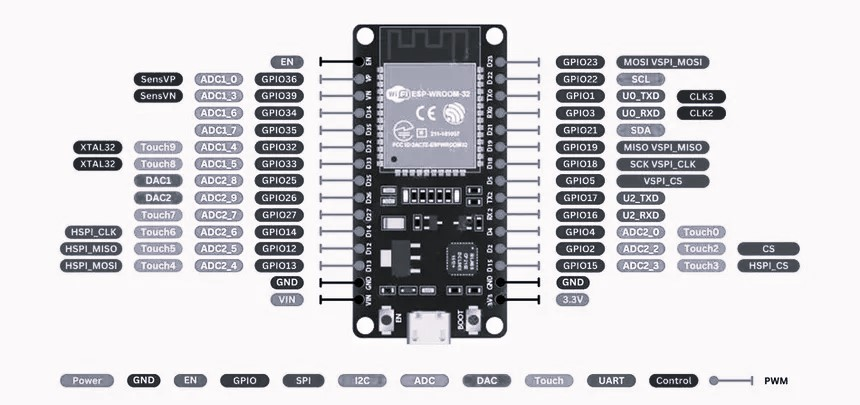
\includegraphics[width=0.5\linewidth]{img/esp32-30pins-pinout.jpg}
    \caption{Pinout do ESP32 de 30 pinos.}
    \label{fig:esp32-pinout}
\end{figure}

\begin{figure}[H]
    \centering
    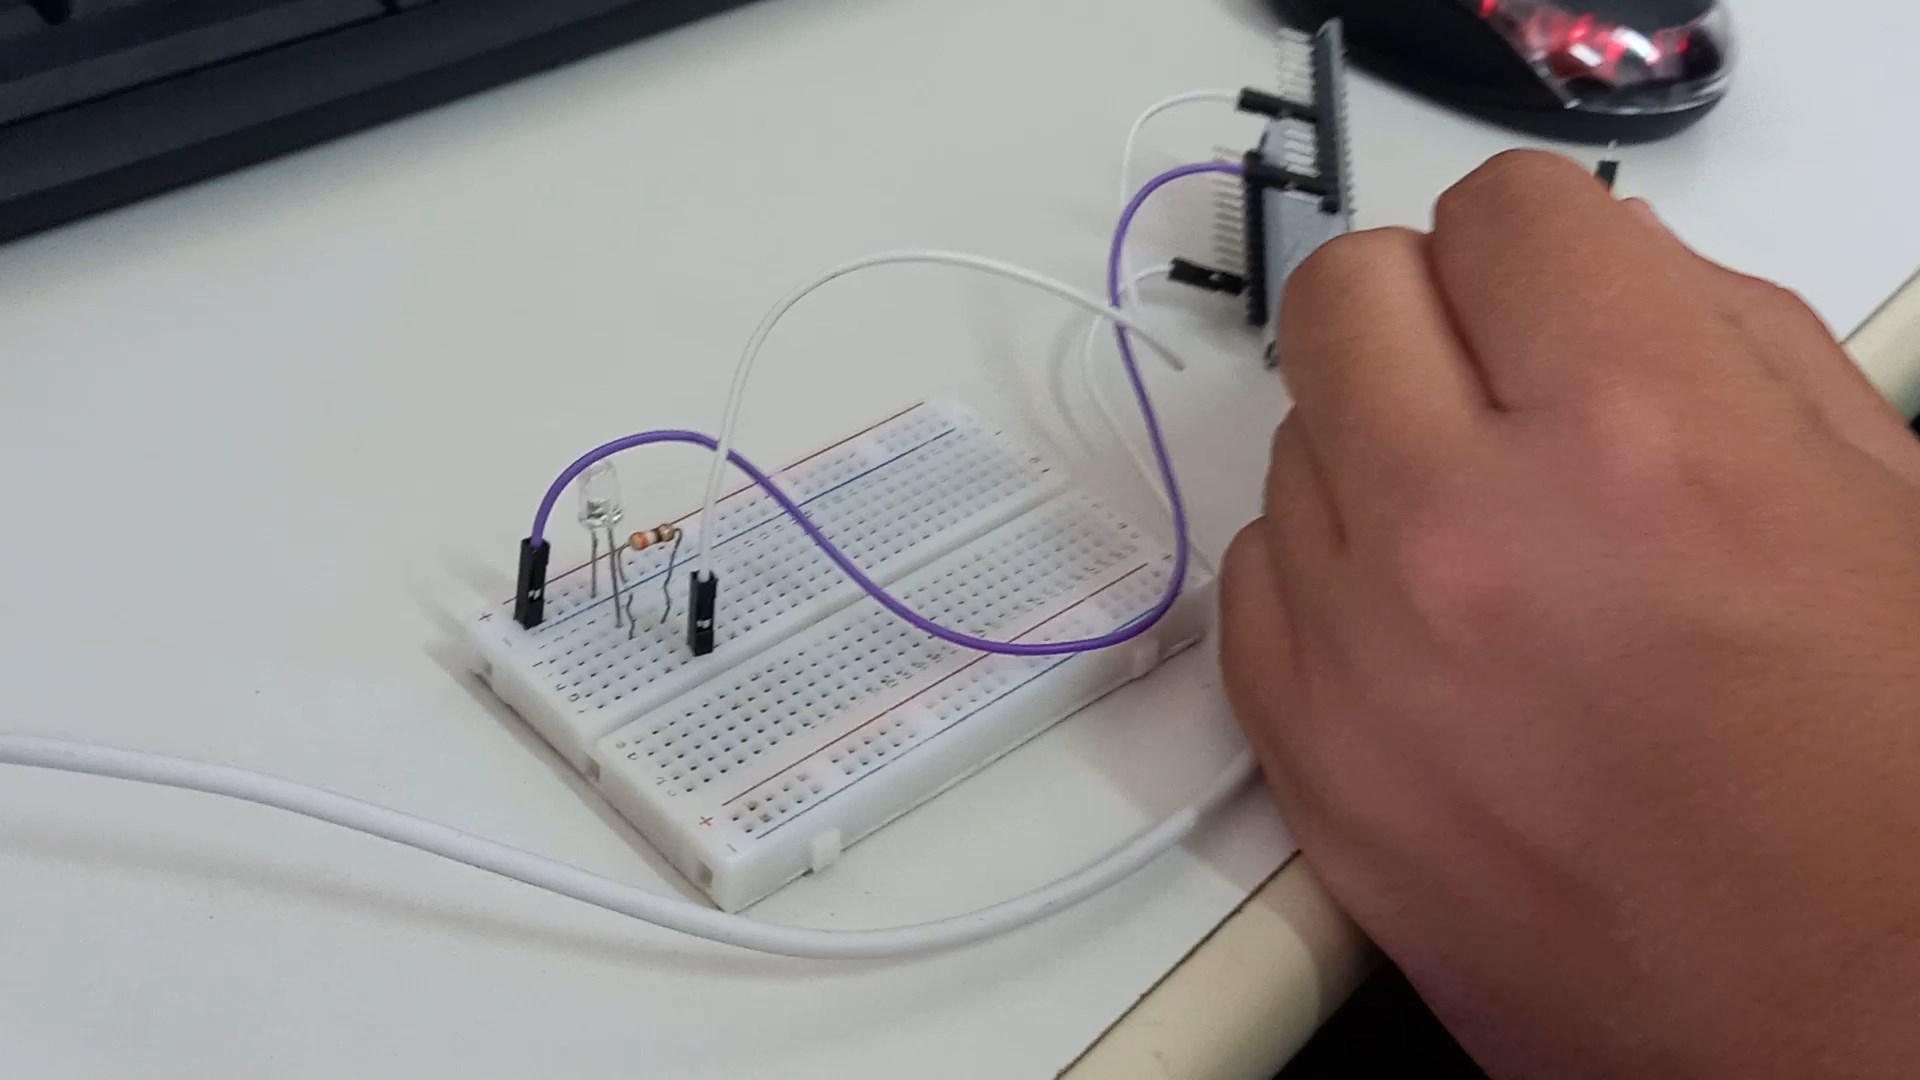
\includegraphics[width=0.5\linewidth]{img/Configuração.jpg}
    \caption{Configuração final na protoboard.}
    \label{fig:protoboard}
\end{figure}

\section{Desenvolvimento do Código}

Não foi necessário instalar nenhuma biblioteca adicional. A biblioteca do Arduino já possui as funções necessárias para colocar o ESP32 para dormir. Apenas, iniciei um novo projeto chamado "Deep Sleep" com o módulo e o framework já comumente usados.

Antes de tudo, vamos configurar o pino do LED. Definimos uma constante LED 25 para representar o pino usado para acender o LED. Em setup, configuramos o pino 25 para modo de saída, e que ele esteja em nível baixo.

\lstinputlisting[language=C++, firstline=14, lastline=15]{code/main.cpp}

E então, configuramos \textit{Deep Sleep}. Primeiro, criamos uma variável global chamada bootCount que irá armazenar a quantidade de vezes que o ESP32 já reiniciou. A variável é acompanhada de \textit{RTC\_DATA\_ATTR} que fará com que a variável seja guardada na memória Real-Time Clock (RTC), fazendo com a variável seja mantida entre as reiniciações.

Outra variável global é o \textit{touchPin} que é do tipo \textit{touch\_pad\_t}. É usado para representar os pinos de \textit{touch} que foram mencionados anteriormente.

\lstinputlisting[language=C++, firstline=7, lastline=8]{code/main.cpp}

Voltando ao \textit{setup}, configuramos o resto da lógica. É preciso lembrar que a cada vez que o ESP32 acorda do \textit{Deep Sleep}, ele executa o \textit{setup} novamente.

Para sabermos quantas vezes o ESP32 já reiniciou, incrementamos a variável bootCount, e imprimos o seu valor no terminou utilizando o método \textit{println} do \textit{Serial}. Foi iniciado o \textit{Serial} no começo do \textit{setup} com a taxa 9600.

\lstinputlisting[language=C++, firstline=18, lastline=18]{code/main.cpp}

Utilizamos a função \textit{esp\_sleep\_get\_touchpad\_wakeup\_status} que retorna o número do pino de \textit{touch} que despertou o ESP32, ou não caso não tenha sido um pino de \textit{touch} que tenha feito o despertar.

\lstinputlisting[language=C++, firstline=21, lastline=21]{code/main.cpp}

É possível utilizar mais de um pino de \textit{touch} e dizemos o que é que deve ser feito no \textit{setup} depois de descobrir qual pino foi tocado. Simplesmente, criamos uma condicional para executar de acordo com o valor que está em \textit{touchPin}. 

O valor que a função anteriormente utilizada retorna não é o número do pino que aparece no \textit{dev kit}, e sim o número do \textit{touch}. Precisamos consultar o \textit{pinout} para saber qual pino aquele número de \textit{touch} representa. No nosso caso, escolhemos o pino 15, que é o pino de \textit{touch} 3.

Dentro do condicional, imprimimos no terminal que o pino 15 foi tocado, configuramos o pino do LED para nível alto e passamos por um pequeno delay de 3 segundos. Colocamos um \textit{else} para indicar que nenhum pino de \textit{touch} foi tocado.

\lstinputlisting[language=C++, firstline=23, lastline=30]{code/main.cpp}

Em seguida, usamos a função \textit{touchSleepWakeUpEnable} para habilitar qum determinado pino a servir como gatilho para acordar o ESP32. Também definimos uma sensibilidade do toque. Definimos uma constante chamada THRESHOLD com valor 40, e para o ESP32, quanto maior o valor, mais sensível é.

O número do pino na função é representado por um "T" mais o número do pino de \textit{touch}.

\lstinputlisting[language=C++, firstline=32, lastline=32]{code/main.cpp}

Antes de fazer o ESP32 dormir, vamos limpar o Serial. Depois, por fim, utilizamos a função \textit{esp\_deep\_sleep\_start} para que o ESP32 caia em \textit{Deep Sleep}.

\lstinputlisting[language=C++, firstline=32, lastline=32]{code/main.cpp}

É possível conferir o código completo nesse \href{https://github.com/fabricio-araujo94/microcontroladores/tree/main/deep_sleep}{repositório no Github}.

\section{Considerações Finais}

O ESP32 é então conectado ao computador, utilizando um cabo microUSB. No Visual Studio Code, apertamos o atalho Alt + Ctrl + U para que o computador envie o código para o ESP32. 

Se estiver no Linux e der erro de permissão em acessar a porta USB, utilize no terminal o comando:

\begin{lstlisting}
sudo chmod 777 /dev/ttyUSB0
\end{lstlisting}

Assim, o ESP32 entrou em sono profundo, e toda vez que o pino de \textit{touch} é tocado, ele desperta e acende o LED, para logo depois, entrar em modo \textit{Deep Sleep} novamente. Fique atento às impressões no terminal para ver se o ESP32 está dormindo ou se ele reconhece o \textit{touch}.

É possível conferir o resultado nesse \href{https://youtu.be/uvPc8xBWX7k}{vídeo no Youtube}.

\begin{figure}[H]
    \centering
    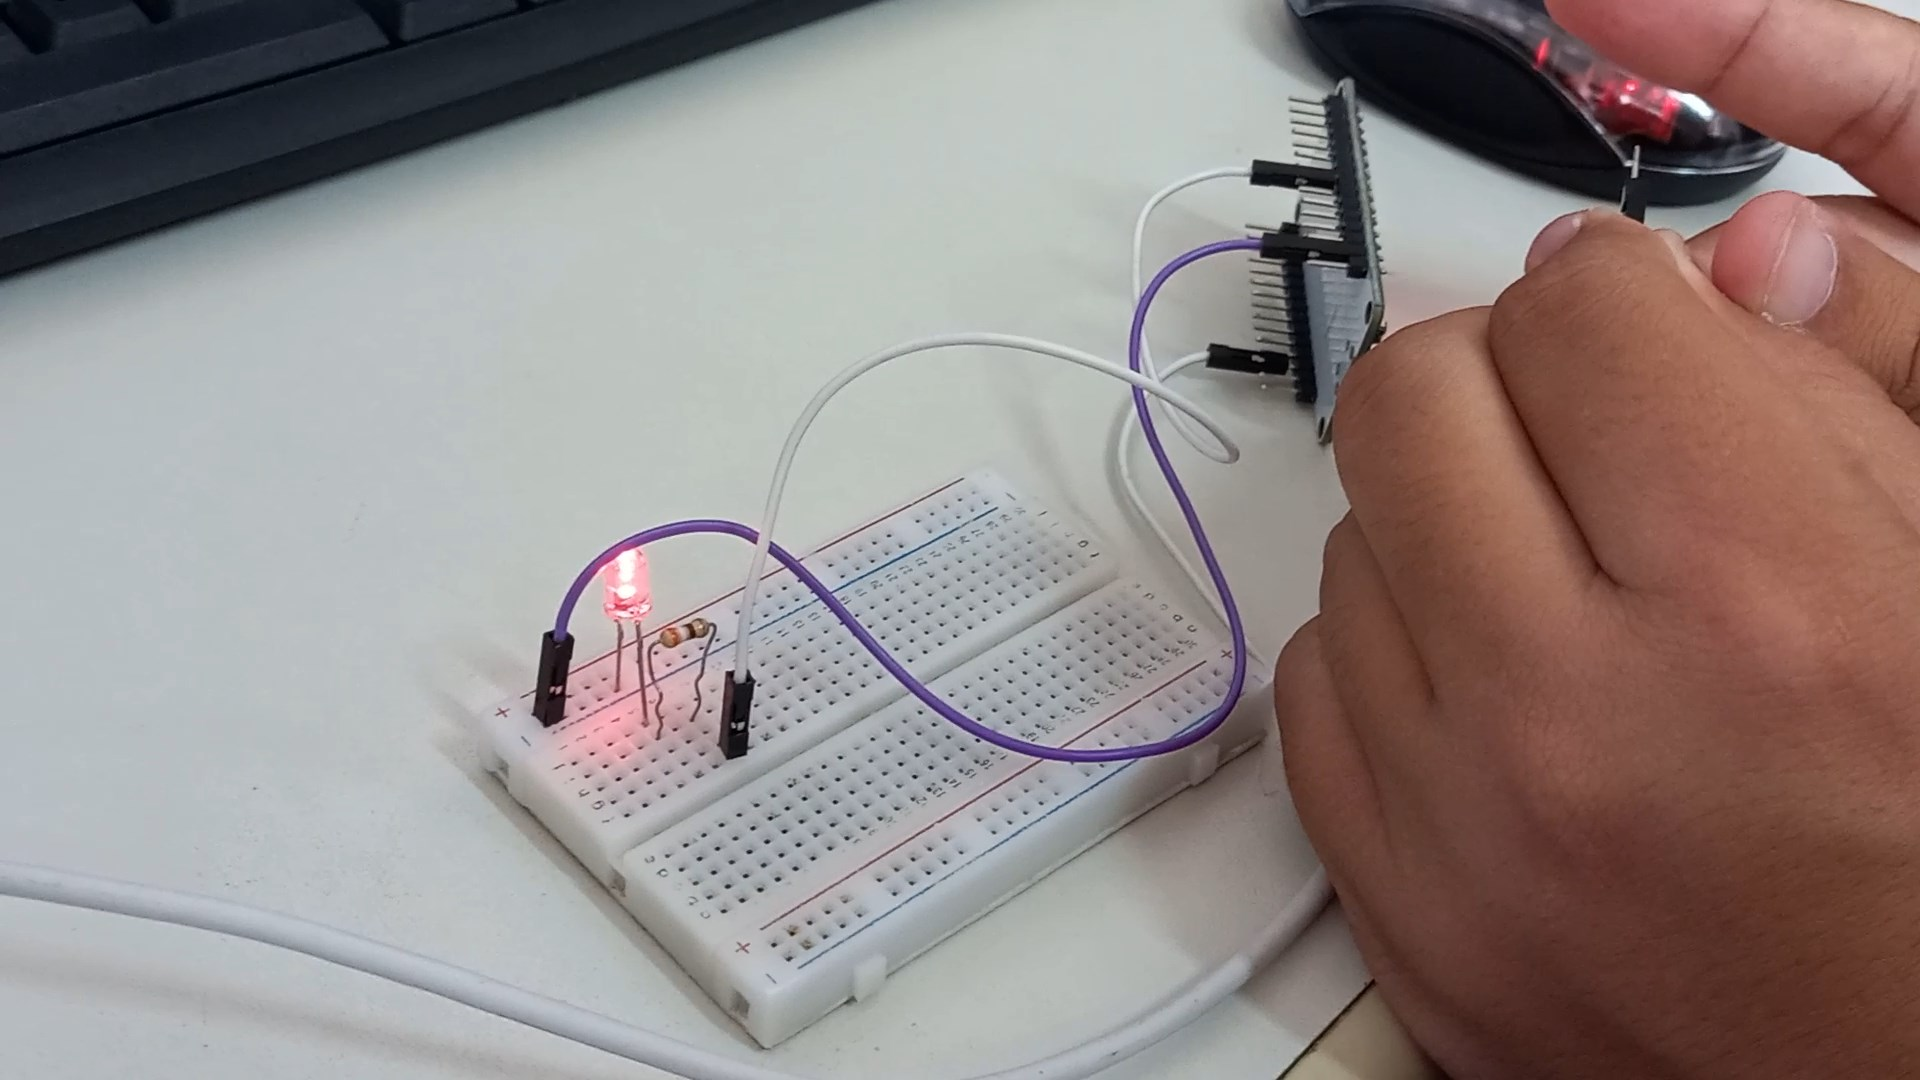
\includegraphics[width=0.5\linewidth]{img/Execução_Protoboart.jpg}
    \caption{Execução na protoboard.}
    \label{fig:protoboard-final}
\end{figure}

\begin{figure}[h]
    \centering
    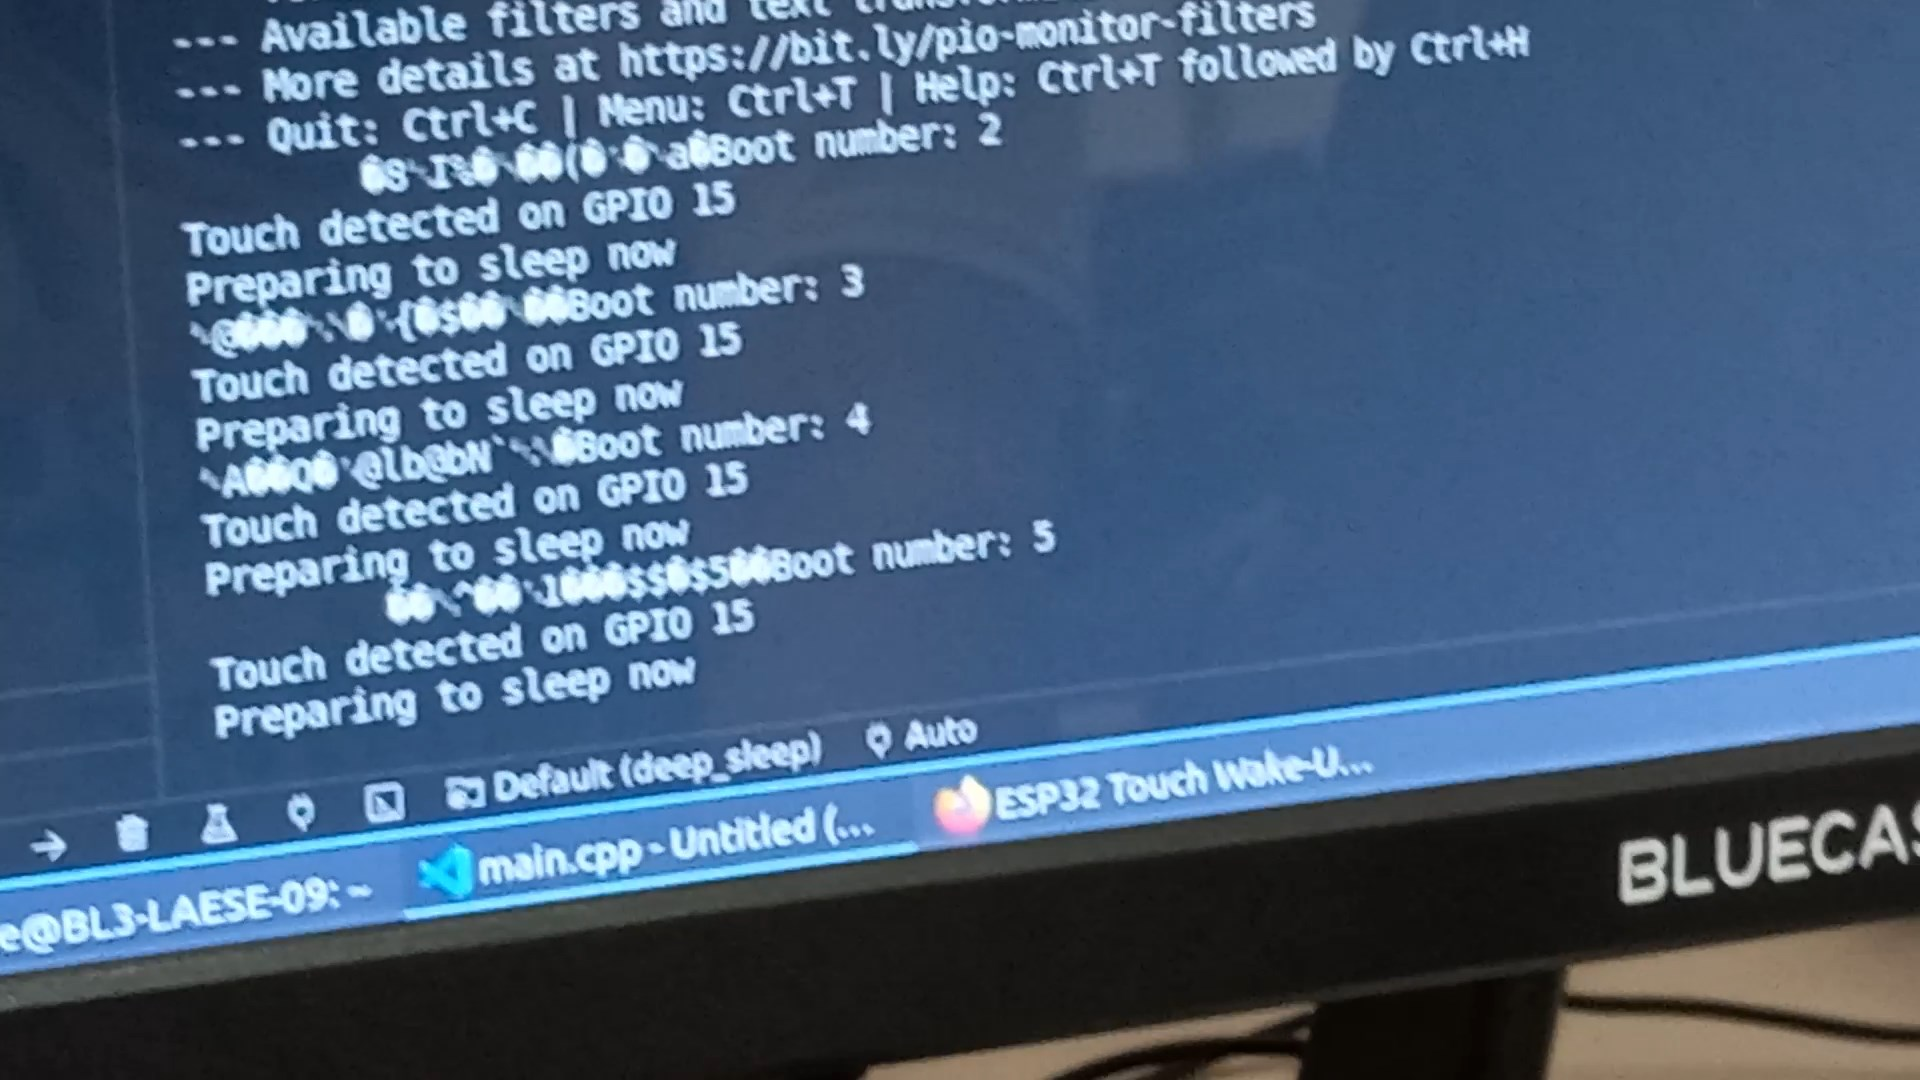
\includegraphics[width=0.5\linewidth]{img/Execução_Terminal.jpg}
    \caption{Execução no terminal.}
    \label{fig:terminal}
\end{figure}

\end{document}
